\section{Sprint 3}

During sprint 3, four variable pitch mechanisms was assembled with Align T-rex 500 RC helicopter tail mechanisms and motors borrowed from HSN. 

\begin{figure}[h]
        \centering
         \begin{minipage}[b]{0.4\textwidth}
            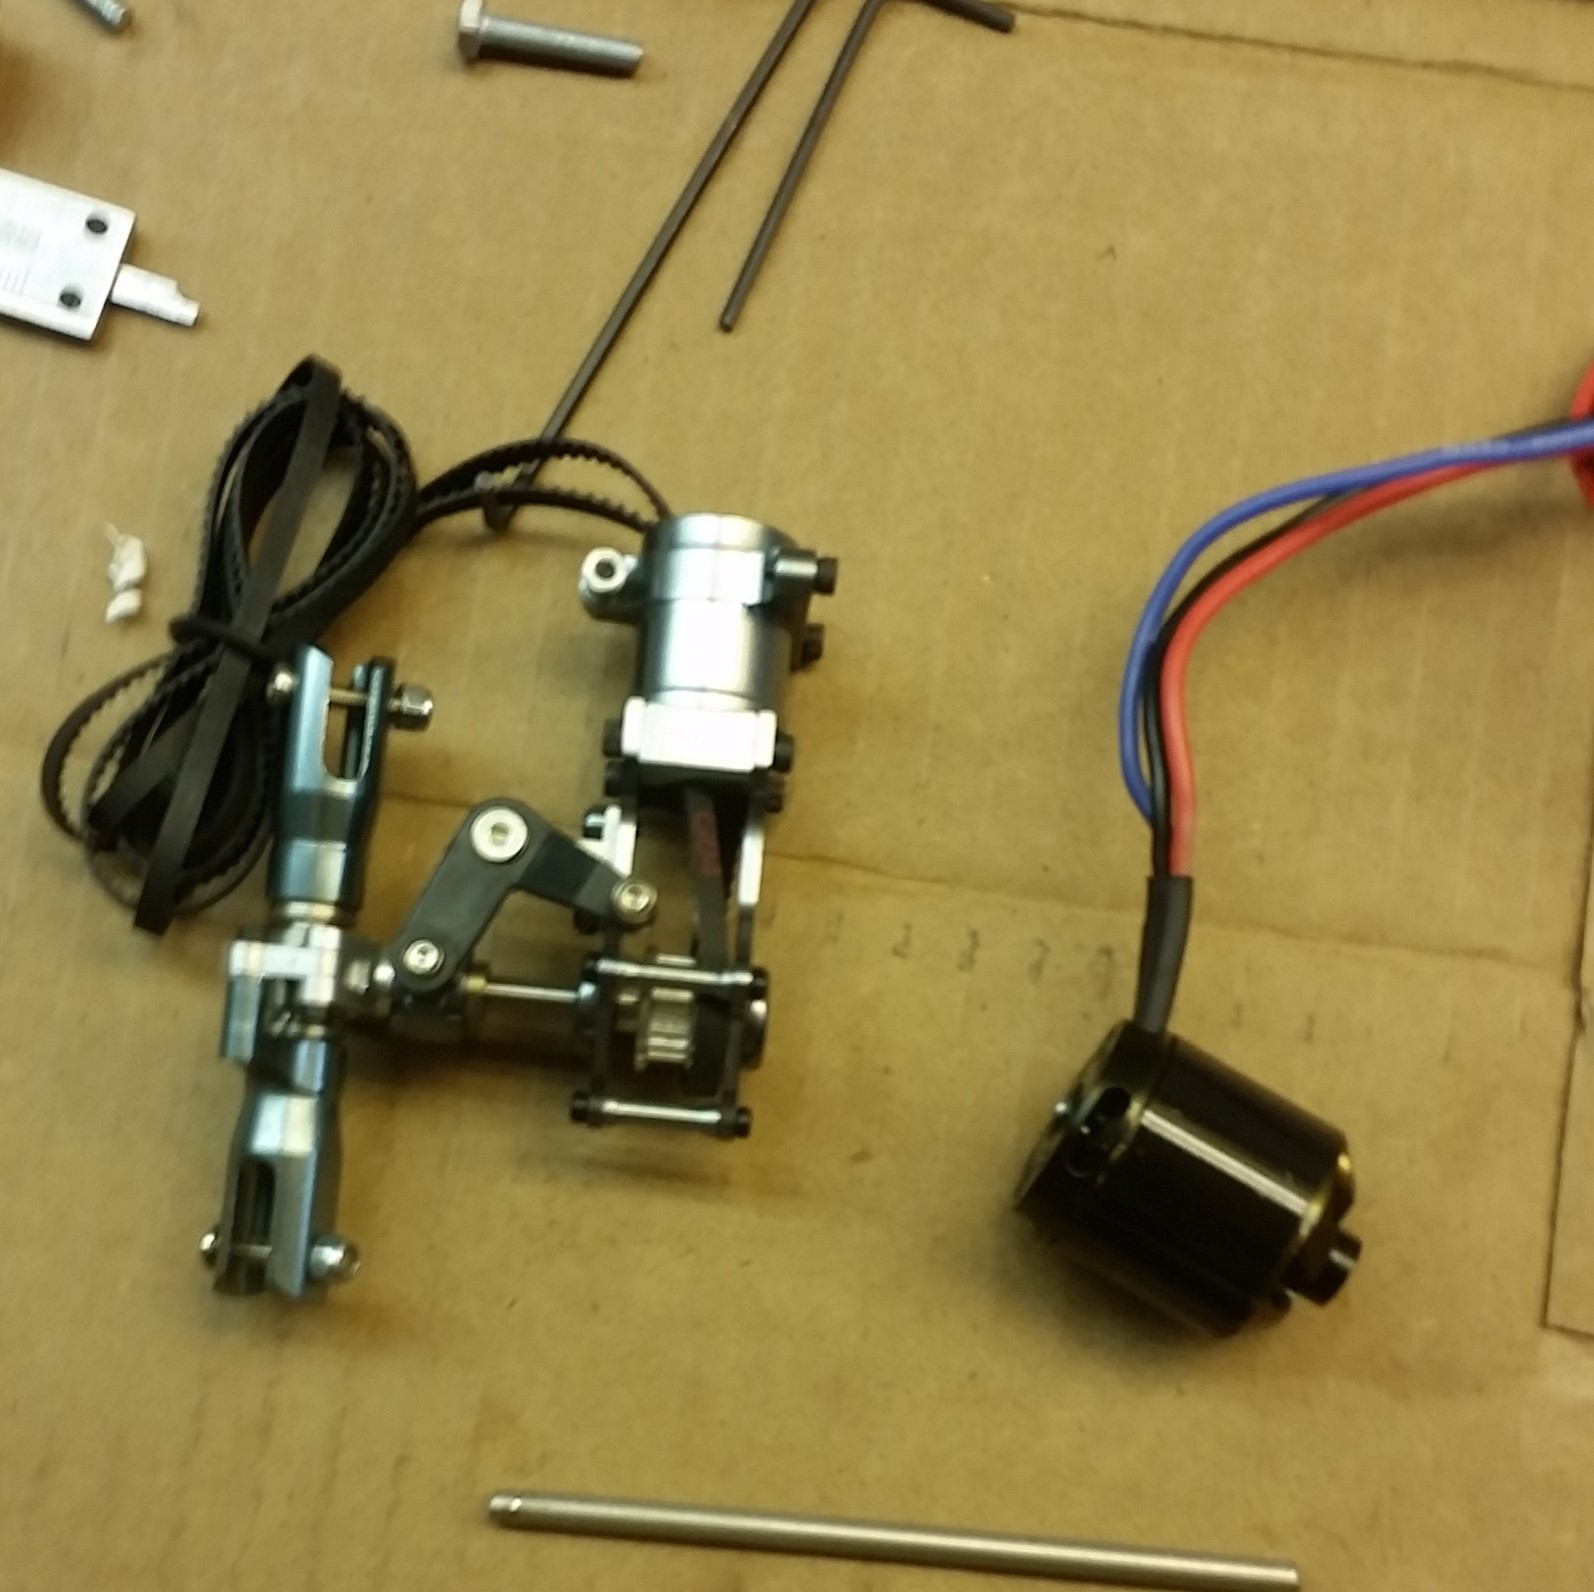
\includegraphics[width = 1\textwidth]{VAPIQ-PICTURES/BeforeAssembly.jpg}
              \caption{Variable Pitch Parts}
            \label{fig:testpic2}
        \end{minipage}
        \hfill
        \begin{minipage}[b]{0.4\textwidth}
            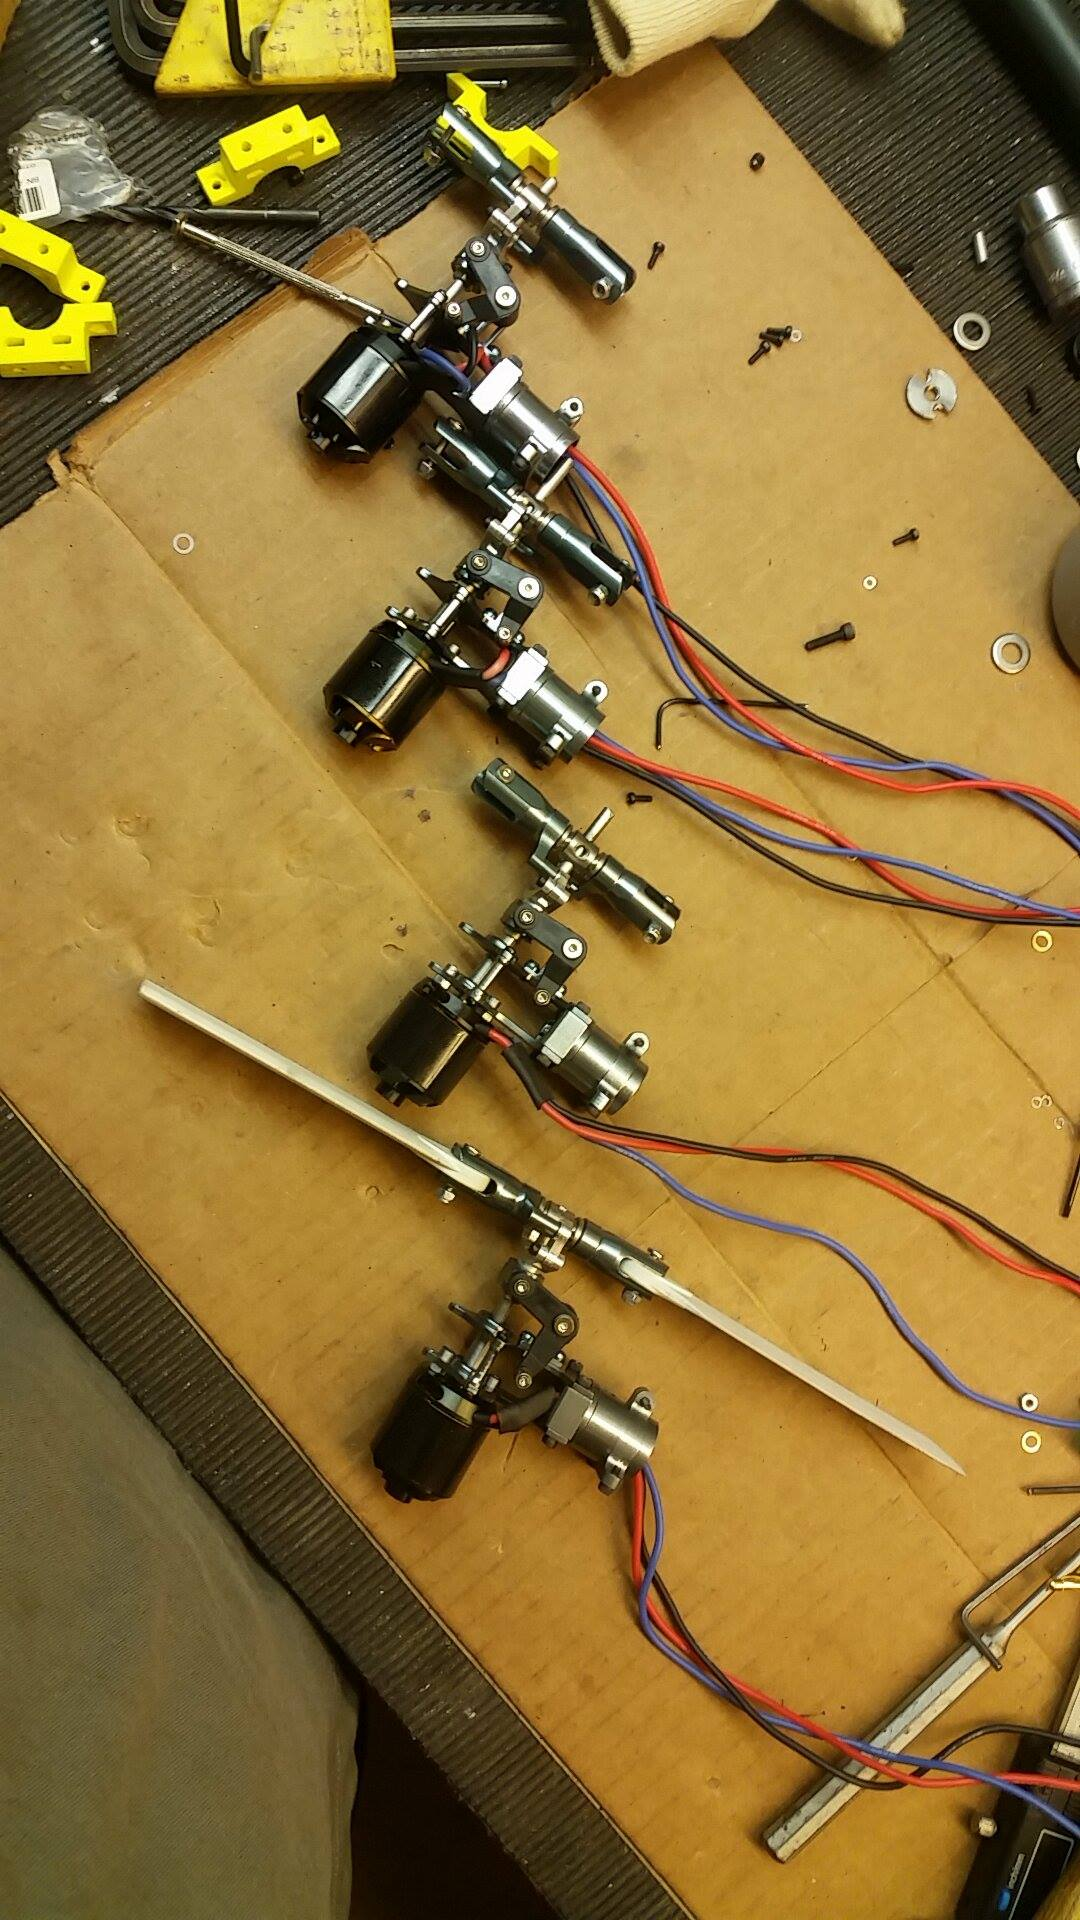
\includegraphics[width = 0.7\textwidth]{VAPIQ-PICTURES/AfterAssemblyVPQ.jpg}
            \caption{Variable Pitch Assembly}
            \label{fig:testpic3}
        \end{minipage}
\end{figure}

We mounted motors from 3dRobotics with 700 KV straight under the mechanism and added symmetric airfoils capable of generating equal amounts of thrust in each direction. The mechanisms function and rotation worked perfectly, but each full assembly with motors, ESC`s, propellers, servos, servo mounts, linkage rods and carbon tubes weighed approximately 250 g. Which for four mechanisms adds up to 1 kg. To build a sufficiently functioning quadcopter thrust to weight should be at least 2:1 as a rule of thumb. Since this is a custom build, it was hard to estimate what lift we could achieve with this motor-propeller assembly theoretically, and the group therefore built a simple thrust test rig which could measure the actual thrust produced. 

\begin{figure}[h]
        \centering
         \begin{minipage}[b]{0.4\textwidth}
            \includegraphics[width = 1\textwidth]{VAPIQ-PICTURES/VPQtestRig}
              \caption{Thrust Test Rig}
            \label{fig:testpic2}
        \end{minipage}
        \hfill
        \begin{minipage}[b]{0.4\textwidth}
            \includegraphics[width = 1\textwidth]{VAPIQ-PICTURES/VpMechanism}
            \caption{Variable Pitch Assembly With Servo}
            \label{fig:testpic3}
        \end{minipage}
\end{figure}


The measured thrust of the motors was approximately 500 g with 3 cell battery voltage and 750 g with four cell voltage. But with four cell voltage and max speed, the motors started to overheat and consumed alot of power 18,6 Amps. On the basis of this information it is not very plausible that this motor- mechanism combination would yield enough lift for this copter, based on the mass budget.

In sprint 3, the group established P-control in one axis in our test rig and established and bluetooth communication with Qualisys. Design wise, there has been generated concepts for fixed pitch. A new design plan for the variable pitch quadcopter had to be made. We also investigated several flight controller options. This includes planning our own setup as well as looking into the possibility of modifying ArduPilotMega or other existing platforms. The biggest problem of using existing flight controllers is the shear amount of code and interdependencies, and the fact that no open-source controller on the market has functionality that supports variable pitch. 

\newpage
\subsection{Completion and Scope Change, Sprint 3}

We have completed 78\% of the planned tasks and had a scope change of 16\%.

Project plan status, sprint 3:


\begin{itemize}
\item Plan Research Paper, \textbf{Started}
\item Mechanical Design Plan, Variabel Pitch, \textbf{Started}
\item Basic Controller, Fixed Pitch, \textbf{Started}
\item Motor Control System, Fixed Pitch, \textbf{Started}
\item Flight Testing And Control, \textbf{Started}
\item Mathematical Model, Variable Pitch, \textbf{Postponed}
\item Electrical Schematic, Fixed Pitch, \textbf{Done}
\item Electrical Schematic, Variabe Pitch, \textbf{Done}
	\end{itemize}


\begin{figure}[h]
        \centering
        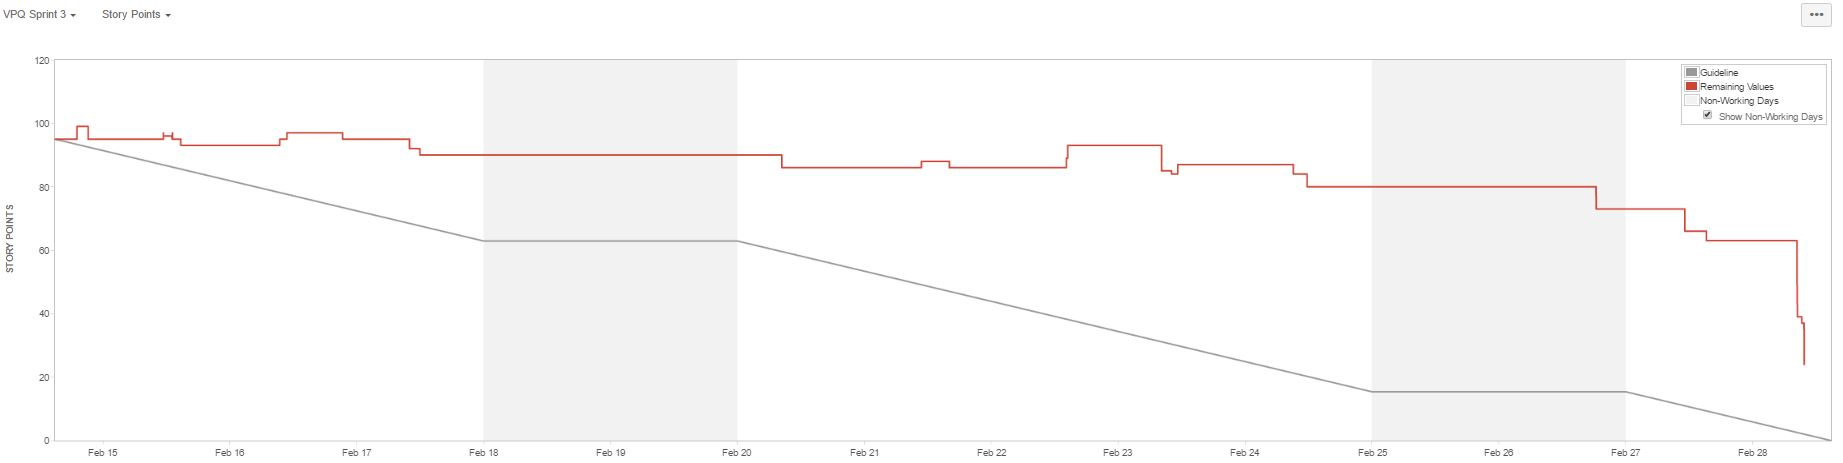
\includegraphics[width = 1\textwidth]{VAPIQ-PICTURES/BDSprint3}
        \caption{Sprint 3}
        \\[2.0 cm]
    \end{figure}
  
\begin{comment}

\subsection{Results and Conclusions}
    
    
    
\subsection{Challenges}




\subsection{Lessons Learned}

\end{comment}    






